\documentclass{article}
\author{李沐辰\ 计卓1501\ U201516994}

\usepackage[UTF8]{ctex}
\usepackage{amsmath}
\usepackage{listings}
\usepackage{xcolor}
\usepackage{graphicx}
\usepackage{geometry} 
\geometry{a4paper,scale=0.8} 
\definecolor{mygreen}{rgb}{0,0.6,0}
\definecolor{mygray}{rgb}{0.5,0.5,0.5}
\definecolor{mymauve}{rgb}{0.58,0,0.82}
\lstset{ %
	backgroundcolor=\color{white},   % choose the background color
	basicstyle=\footnotesize\ttfamily,        % size of fonts used for the code
	columns=fullflexible,
	breaklines=true,                 % automatic line breaking only at whitespace
	captionpos=b,                    % sets the caption-position to bottom
	tabsize=4,
	commentstyle=\color{mygreen},    % comment style
	escapeinside={\%*}{*)},          % if you want to add LaTeX within your code
	keywordstyle=\color{blue},       % keyword style
	stringstyle=\color{mymauve}\ttfamily,     % string literal style
	frame=single,
	rulesepcolor=\color{red!20!green!20!blue!20},
	% identifierstyle=\color{red},
	language=c++,
}

\title{从$\lambda$演算到并行——函数式的前世今生}
\date{}
\begin{document}
	\maketitle
	函数式编程是一种编程典范。最早可以追溯到上世纪三十年代。从1958年lisp的诞生以来,到1980年haskell发布,如今出现越来越多的函数式编程语言,函数式编程思想也越来越多的被主流编程语言所采用如Java,python等如今都有与函数式编程有关的语法。在未来程序并行化的趋势下,函数式编程思想的优势也让它脱颖而出收到越来越多的关注。
	\section{数学起源——$\lambda$演算}
	函数式编程起源于$\lambda$演算,$\lambda$演算可以说是函数式编程思想的思想基础,那$\lambda$演算究竟是一个什么东西呢
	\subsection{直觉化描述}
	$\lambda$演算($\lambda$calculus)是一套从数学逻辑中发展,以变量绑定和替换的规则,来研究函数如何抽象化定义、函数如何被应用以及递归的形式系统。它由数学家阿隆佐·邱奇在20世纪30年代首次发表。Lambda演算作为一种广泛用途的计算模型,可以清晰地定义什么是一个可计算函数,而任何可计算函数都能以这种形式表达和求值,它能模拟单一磁带图灵机的计算过程;尽管如此,Lambda演算强调的是变换规则的运用,而非实现它们的具体机器。
	
	这么一看,$\lambda$演算可是一个很强大的工具,由于它包含规则替换和函数抽象化定义的方式,它完全可以看做是一个最根本的编程语言。
	
	在$\lambda$演算中,每个表达式都代表一个函数,这个函数有一个参数,并且会返回一个值。不论是参数和返回值,也都是一个单参的函数。可以这么说,$\lambda$演算中只有一种“类型”,那就是这种单参函数。函数是通过λ表达式匿名地定义的,这个表达式说明了此函数将对其参数进行什么操作。
	\subsection{形式化描述}
	$\lambda$演算的语法可以简化为如下三条,其实是一个BNF范式表达的上下文无关文法。
	\begin{enumerate}
	\item <表达式> ::= <标识符>
	\item <表达式> ::= ($\lambda$<标识符>.<表达式>)
	\item <表达式> ::= (<表达式> <表达式>)
	\end{enumerate}
	前两条规则主要目的是用来生成函数,第三条描述了函数是如何作用在参数上的。
	\subsection{$\lambda$演算与其可计算性}
	$\lambda$运算当中有大量的数学思想,特别是函数为一等公民的核心性质,重新定义了我们平时所熟悉的很多内容,例如bool值,甚至自然数等,都可以用函数进行定义,具体较为抽象,下面我们从几个简单的例子展示一下$\lambda$演算的强大力量
	
		\subsubsection{函数生成器}
		简单的来说$\lambda$演算有两个主要的公理
		\begin{itemize}
		\item $\lambda\ x\ y.\ x+y => \lambda\ a\ b.\ a+b$ (*置换公理*)
		\item $(\lambda\ x\ y.\ x+y)\ a\ b=>a+b$	(*带入公理*)
		\end{itemize}
	
		可见$\lambda$表达式函数之间可以调用替换,相当于一个函数生成器
		
		我们可以考虑更多的例子
		\begin{enumerate}
		\item 
			考虑not函数,定义:
			
			$let\ not = $
			\begin{itemize}
				\item  $false -> true$
				\item  $true -> false$
			\end{itemize}
			
			其它逻辑函数类似,考虑不同的情况即可
		\item
			广义的and函数:
			
			$let\ and =$ 
			\begin{itemize}
				\item $true\ value -> value$
				\item $false\ value -> false$
				\item $value\ true -> value$
				\item $value\ false -> false$
			\end{itemize}
		
		\item
			考虑if
			
			$let\ if =$ 
			
			$\lambda\ cond\ tvalue\ fvalue.\ (cond\ and\ tvalue)\ or\ (not\ cond\ and\ fvalue)$
			
			$if\ true\ a\ b$试着展开看看:
			\begin{itemize}
				\item  $-> (true\ and\ a)\ or\ (false\ and\ b)$
				\item  $-> a\ or\ false$
				\item  $-> a$
			\end{itemize}
		\end{enumerate}
	
		\subsubsection{解决递归}
		在函数生成器的例子当中我们看到了,函数可以调用其它函数。假设我们遇到一个问题它要求定义一个函数计算前n个数的和。考虑如下定义
		
		\begin{itemize}
			\item $let\ sumn=\lambda\ n\ .\ if\ (n==1)\ 1\ (n + sumn\ n-1)$
		\end{itemize}
	
		在定义fact的同时我们引用到了自身,这种写法在编程当中虽然很常见,但是并不能被数学体系所接受。
		
		一种解决方法是将函数自身作为参数传入,不过这种方法有点耍赖皮了,因为它不是真正的递归,只是使用参数将函数自身也传入而已
		\begin{itemize}
			\item $let\ P = \lambda\ self\ n.\ if\ (n == 0)\ 1\ (n+self(self\ n-1))$
			\item $let\ fact\ n\ =\ P\ (P\ n)$
		\end{itemize}
		我们先来看一个有趣的$\lambda$表达式: 
		$$\omega = \lambda\ x.\ x\ x$$
		当我们让$\omega$函数作用于自身身上,将其按规则展开
		$$\omega\ \omega = (\lambda\ x.\ x\ x)\ \omega = \omega\ \omega$$
		发现展开后又还原回来,我们发现这里函数作用中存在某种不变性,从这个角度可以引出不动点定理的证明
		
		具体考虑这样一个组合子
		$$Let\ Y = \lambda\ F.\ (\lambda\ x.\ F(x\ x))\ (\lambda\ x.\ F(x\ x))$$
		这里再次应用了两次作用自身的技巧其中令$a = \lambda\ x.\ F(x\ x)$则有$Y = \lambda\ F.\ a\ a$
		
		带入任意函数a
		\begin{equation}
		\begin{split}
		Y\ g & =  a\ a \\
			 & = (\lambda\ x.\ g(x\ x))\ a \\
			 & = g(a\ a)\\
			 & = g\ (Y\ g)
		\end{split}
		\end{equation}
		上式实际上证明了\textbf{不定点定理},其内容为
		\textbf{对于任意$\lambda$表达式$g$,总存在不动点$x = Y\ g$,使关系$g\ x = x$成立}
		
		有了上述的结论,我们回到一开始的问题,为前n项求和的函数生成一个递归的表达式。
		$let\ P = \lambda\ self\ n.\ if\ (n==1)\ 1\ (n+self\ n-1)$并且根据(1)有		
		\begin{equation}
		\begin{split}
		Y (P)& =  a\ a \\
			& = P\ (a\ a)\\
			& = if\ (n==1)\ 1\ (n+Y(P)\ n-1)
		\end{split}
		\end{equation}
		根据(2),很明显我们得到了一个递归结构的程序!$let\ sumn=Y(P)$,显然$sumn$就是我们一开始想要的递归程序!
		
		\subsubsection{图灵完备性}
		$\lambda$演算可以推导出新的函数,根据不定点定理可以解决函数形式的递归。具备了递归函数的构造能力,依据可计算性理论,$\lambda$演算体系便构成了图灵完备系统,这是一个很令人振奋的结论。所谓图灵完备系统,概括而论即任何可计算的函数,均可由此系统来构造。这个结论表明,$\lambda$演算体系能够做到当前通用计算机所能够做到的一切。
		
		举一个用$\lambda$演算转换问题的例子,考虑一个经典的停机问题,即不可判定一个图灵机在给定任意输入的时候是否可以停机。这个命题在$\lambda$演算中的等价命题是:不存在一个算法能够判定任意两个$\lambda$函数是否等价,即对于所有的$n$,有$f(n)=g(n)$。

	\section{函数式编程的现代发展}
	函数式编程发展到今天,越来越多的主流语言开始吸收函数式编程的思想,开始支持函数式编程风格
	\subsection{特性}
		函数式编程实际上是一种编程范式,其它常见的还有命令式编程。对比命令式编程,函数式并不那么关心执行的流程而是关心数据的映射。相对的,我理解的函数式编程是对所要解决问题的一个高度抽象,一等公民函数实际上是从问题输入到问题解的一个映射,而不是对其流程的描述。
		
		命令式编程是面向计算机硬件的抽象,有变量(对应着存储单元),赋值语句(获取,存储指令),表达式(内存引用和算术运算)和控制语句(跳转指令),一句话,命令式程序就是一个冯诺依曼机的指令序列。而函数式编程是面向数学的抽象,将计算描述为一种表达式求值,一句话,函数式程序就是一个表达式。
		
		令函数式编程独特的性质主要有以下几点:
		
		\begin{enumerate}
			\item 不可变性
			
			函数式编程当中区别于命令式编程当中的概念,不代表储存单元,而是表示数学当中的变量,因而不能够多次赋值。这也带来了巨大的好处,即函数不会改变状态,程序员不用再费心维护函数中的状态。
			
			\item 函数作为一等公民
			
			这个技术可以让你的函数就像变量一样来使用。也就是说,你的函数可以像变量一样被创建,修改,并当成变量一样传递,返回或是在函数中嵌套函数。因而就有了高阶函数
			
			\item 尾递归优化
			
			递归更符合人的思维方式,同时对于用递归描述的程序,为了提高其的性能,使用尾递归优化技术,每次递归时都会重用stack。
		\end{enumerate}
	
	\subsection{Python 视角}
	python作为一门多范式的现代语言,其实仔细分析,其很多特性吸取了函数式编程中的思想。这里据一些例子分析。
		\subsubsection{lambda 表达式与 map \& reduce}
		高阶函数可以接收函数做参数,有些时候,我们不需要显式地定义函数,直接传入匿名函数更方便。而python当中的lambda表达式就为这一特性提供了基础。
		
		map()是 Python 内置的高阶函数,它接收一个函数 f 和一个 list,并通过把函数 f 依次作用在 list 的每个元素上,得到一个新的 list 并返回。
		
		reduce()函数也是Python内置的一个高阶函数。reduce()函数接收的参数和 map()类似,一个函数 f,一个list,但行为和 map()不同,reduce()传入的函数 f 必须接收两个参数,reduce()对list的每个元素反复调用函数f,并返回最终结果值。
		
		综合利用lambda表达式和map \& reduce可以大大简化python的代码编写,也让代码流程变得清晰。
		
		\lstset{language=python}
		\begin{lstlisting}
map(lambda x: x * x, [1, 2, 3, 4, 5, 6, 7, 8, 9])
		\end{lstlisting}
		
		高阶函数map, 接受一个匿名函数作为输入,输出列表中每个元素平方输出的列表。
		同样的高阶函数还有filter\&sort等
		
		\subsubsection{pipeline与惰性求值}
		pipeline 管道借鉴于Unix Shell的管道操作——把若干个命令串起来,前面命令的输出成为后面命令的输入,如此完成一个流式计算。
		
		参考如下程序
		\lstset{language=python}
		\begin{lstlisting}
def multiply_by_three(nums):
	for num in nums:
		yield num * 3
def convert_to_string(nums):
	for num in nums:
		yield 'The Number:%s' % num
nums = [1, 2, 3, 4, 5, 6, 7, 8, 9, 10]
pipeline = convert_to_string(multiply_by_three(nums))
for num in pipeline:
	print num
		\end{lstlisting}
		
		我们动用了Python的关键字 yield,这个关键字主要是返回一个Generator,yield 是一个类似return的关键字,只是这个函数返回的是个Generator-生成器。所谓生成器的意思是,yield返回的是一个可迭代的对象,并没有真正的执行函数。也就是说,只有其返回的迭代对象被真正迭代时,yield函数才会正真的运行,运行到yield语句时就会停住,然后等下一次的迭代。(这个是个比较诡异的关键字)这实际上就是惰性求值的思想。
		\subsubsection{decorator 与高阶函数}
		如果想要在运行式给一个写好的函数增加行为,又不想改动原函数,在函数式编程里面我们可以用原函数去生成新的函数,对应于python当中,我们可以用装饰器(decorator)来解决这个问题。
		
		Python的 decorator 本质上就是一个高阶函数,它接收一个函数作为参数,然后,返回一个新函数。
		
		\lstset{language=python}
		\begin{lstlisting}
def log(f):
	# 使用*args以解决多参数
	def fn(*args, **kw):
		print 'call ' + f.__name__ + '()...'
		return f(*args, **kw)
	return fn

@log
def add(x, y):
	return x + y
print add(1, 2)
		\end{lstlisting}
		对于接受参数的decorator来说则是又加了一层高阶函数,参考如下代码,可以动态指定每次log的开头
		
		\lstset{language=python}
		\begin{lstlisting}
def log(prefix):
	def log_decorator(f):
		def wrapper(*args, **kw):
			print '[%s] %s()...' % (prefix, f.__name__)
			return f(*args, **kw)
		return wrapper
	return log_decorator

@log('DEBUG')
def test():
	pass
print test()
		\end{lstlisting}
		
		\subsubsection{闭包与函数作为返回值}
		python中在函数内部定义的函数和外部定义的函数是一样的,只是他们无法被外部访问。内层函数引用了外层函数的变量(参数也算变量),然后返回内层函数的情况,称为\textbf{闭包(Closure)}。
		
		闭包的特点是返回的函数还引用了外层函数的局部变量,所以,要正确使用闭包,就要\textbf{确保引用的局部变量在函数返回后不能变}。
		
\lstset{language=python}
\begin{lstlisting}
# 希望一次返回3个函数,分别计算1x1,2x2,3x3:
def count():
	fs = []
	for i in range(1, 4):
		def f():	
			return i*i		
	fs.append(f)
	return fs

f1, f2, f3 = count()
# Output: 9 ,9 ,9
\end{lstlisting}
		输出999原因就是当count()函数返回了3个函数时,这3个函数所引用的变量 i 的值已经变成了3。由于f1、f2、f3并没有被调用,所以,此时他们并未计算 i*i,当 f1 被调用时,i=3,返回i*i=9

\lstset{language=python}
\begin{lstlisting}
# 希望一次返回3个函数,分别计算1x1,2x2,3x3:
def count():
	fs = []
	for i in range(1, 4):
		def f():	
			return (lambda : i*i)		
		fs.append(f)
	return fs

f1, f2, f3 = count()
# Output: 9 ,9 ,9
\end{lstlisting}
		上面的lambda表达式定义了一个匿名函数,实际上是返回了一个常数值,这个常数值由每一次迭代时的i决定。
	
	\section{函数式的并行化优势与挑战}
		前面也有提到过,函数式有高阶函数的特性,但由于命令式计算也可以通过类似指针的方法来实现高阶函数,函数式的最主要的好处主要是由不可变性带来的,没有可变的状态,函数就是\textbf{引用透明}的。
		
		一个好处是,函数即不依赖外部的状态也不修改外部的状态,函数调用的结果不依赖调用的时间和位置,这样写的代码容易进行推理,不容易出错。这使得单元测试和调试都更容易。
		
		不变性带来的另一个好处是:由于(多个线程之间)不共享状态,不会造成资源争用(Race condition),也就不需要用锁来保护可变状态,也就不会出现死锁,这样可以更好地并发起来,尤其是在对称多处理器(SMP)架构下能够更好地利用多个处理器(核)提供的并行处理能力。
		
		如同图1所给出的,2005年以来CPU的主频增长(蓝线)已经到达一个瓶颈,支持着CPU计算能力增长的因素转变为CPU核数的增多。
		
		\begin{figure}[ht]
			\centering
			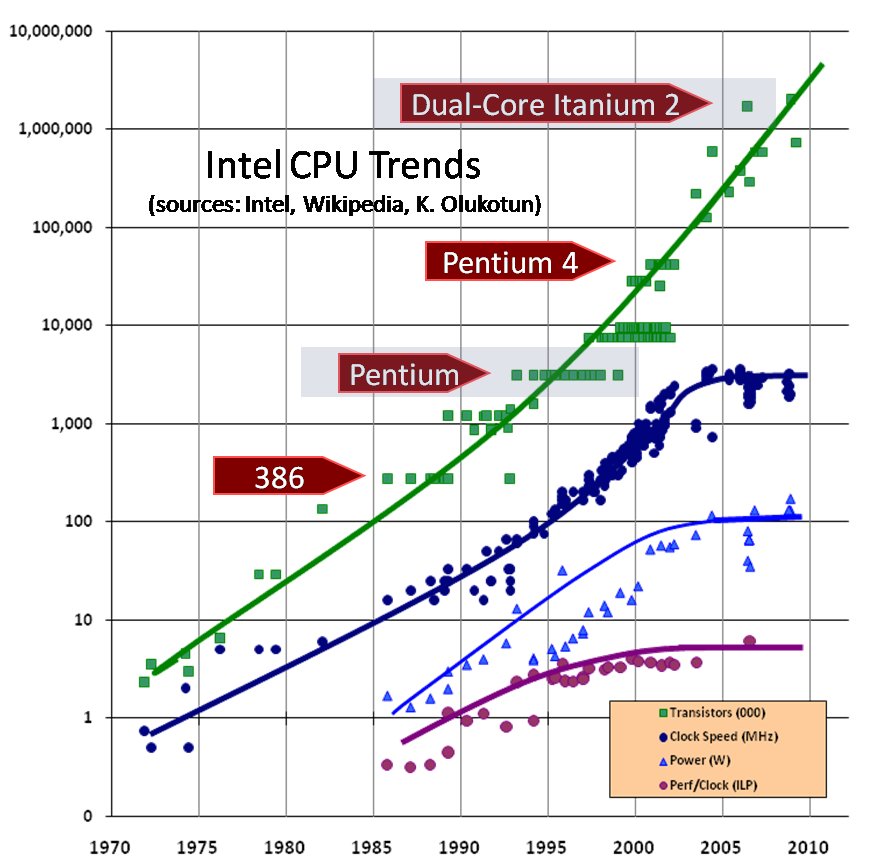
\includegraphics[scale=0.6]{CPU.png}
			\caption{Intel CPU Introductions (graph updated August 2009; article text original from December 2004)}
			\label{fig:label}
		\end{figure}
	
		在多核或多处理器的环境下的程序设计是很困难的,难点就是在于共享的可变状态。在这一背景下,这个好处就有非常重要的意义。 
		
		由于函数是引用透明的,以及函数式编程不像命令式编程那样关注执行步骤,这个系统提供了优化函数式程序的空间,包括惰性求值和并性处理。函数式编程自然在未来并行化的发展方向上有巨大的优势
	
\end{document}